\newpage
\subsection{Full House}
\label{Full_House}
Wenn in einer Figur 8 Zahlen eingetragen sind, dann kann die Technik \textit{Full House} angewendet werden. Da in jeder Figur die Zahlen 1 bis 9 stehen müssen, kann die fehlende Zahl einfach per Ausschluss ermittelt werden.\\

\begin{figure}[h]
\begin{center}
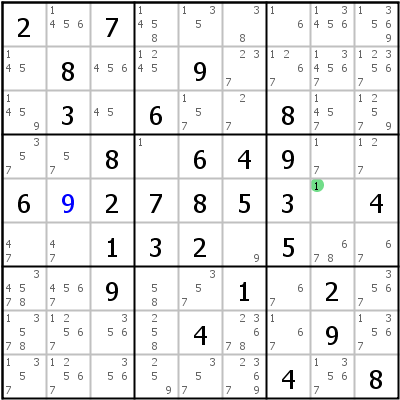
\includegraphics{./img/full_house.png}
\caption{Full House}
\end{center}
\end{figure}

In \textbf{Abbildung 3.1} fehlt in Zeile 5 nur noch eine Ziffer. Da die Zahlen 2 bis 9 bereits vorhanden sind, kann in das Feld z5s8 die Zahl 1 eingetragen werden.